
\section{空间解析几何}

\subsection*{Linear Algebra and Analytic Geometry}

\subsubsection{Inner Product}

Let $V$ be a real vector space. An inner product on $V$ is a map
\begin{align*}
    g: V \times V & \to \mathbb{R}  \\
    (u, w)        & \mapsto g(u, w)
\end{align*}
satisfying
\begin{enumerate}
    \item \allbold{Bi}linearity:\\
          $g(\lambda_1v_1+\lambda_2v_2,w)=\lambda_1g(v_1,w)+\lambda_2g(v_2,w)$\\
          $g(v, \lambda_1w_1+\lambda_2w_2)=\lambda_1g(v,w_1)+\lambda_2g(v,w_2)$
    \item Symmetry: $g(v,w)=g(w,v)$ for all $(v,w)\in V$
    \item Positive definite 正定: $g(v,v)\geq 0$ for all $v\in V$, with equality iff $v=0$
\end{enumerate}

An inner product is also denoted by $\langle\cdot,\cdot\rangle_g$, or $\langle\cdot,\cdot\rangle$, or ``$\cdot$'' if there is no confusion.

\begin{example}
    $V=C[0,1],\,\langle f,g\rangle\triangleq\int_0^1 f(x)g(x)\,\mathrm{d}x$
\end{example}

For $\dim_{\mathbb{R}}V=n<+\infty$, we have the following classification results.

\begin{theorem}[Classification of \allbold{Symmetric Bilinear Form}]
    If $\dim_{\mathbb{R}}V=n$, then for any symmetric bilinear form $g$ on $V$, there exists a basis $\left(v_1,\dots,v_n\right)$ such that
    $$
        \left(g\left(v_i,v_j\right)\right)_{1\leq i,j\leq n}=
        \begin{bmatrix}
            1 &        &   &    &        &    &   &        &   \\
              & \ddots &   &    &        &    &   &        &   \\
              &        & 1 &    &        &    &   &        &   \\
              &        &   & -1 &        &    &   &        &   \\
              &        &   &    & \ddots &    &   &        &   \\
              &        &   &    &        & -1 &   &        &   \\
              &        &   &    &        &    & 0 &        &   \\
              &        &   &    &        &    &   & \ddots &   \\
              &        &   &    &        &    &   &        & 0
        \end{bmatrix}(\text{$r_+$个$1$，$r_-$个$-1$，$n-r_+-r_-$个$0$})
    $$
    where $r_+=\max\left\{\dim_{\mathbb{R}}W\mid g|_W>0\text{ on a subspace }W\right\}$, and $r_-$ is defined similarly.

    These are called the positive and negative inertia indices, respectively.
\end{theorem}

\begin{theorem}[Classification of Inner Product]
    If $\dim_{\mathbb{R}}V=n$, then for any inner product $g$ on $V$,
    \begin{enumerate}
        \item there exists a basis $\left(v_1,\dots,v_n\right)$ such that
              $$\left(g\left(v_i,v_j\right)\right)=\begin{pmatrix}
                      1 &  & \\&\ddots&\\&&1
                  \end{pmatrix},\,\text{i.e. }g\left(v_i,v_j\right)=\delta_{ij}=\begin{cases}
                      1 & i=j \\0&i\neq j
                  \end{cases}(\text{\allbold{Kronecker Symbol}})$$
              i.e. an orthonormal basis with respect to $g$ exists.
        \item any basis $\left(v_1',\dots,v_n'\right)$ is orthonormal with respect to $g$ iff
              $$\left(v_1',\dots,v_n'\right)=\left(v_1,\dots,v_n\right)P$$
              for some $P\in O(n)=\left\{A\in M_{n\times n}(\mathbb{R})\mid AA^T=I\right\}$, \allbold{called the orthogonal group 正交群}.
    \end{enumerate}
\end{theorem}

In coordinates:

Let $V$ be an $n$-dimensional real vector space. An ordered set of $n$ linearly independent vectors is called an ordered basis, usually denoted by $(v_1,\dots,v_n)$.

Fix a particular ordered basis $(v_1,\dots,v_n)$. We then have the following one-to-one correspondences.

\begin{enumerate}
    \item $V\to\mathbb{R}^n$ \allbold{isomorphism 同构}\\
          $v\to x=\begin{pmatrix}
                  x_1 \\\vdots\\x_n
              \end{pmatrix}$ \allbold{coordinate vector (w.r.t. the ordered basis $v_1,\dotsm,v_n$)}\\
          such that $v=\begin{pmatrix}
                  v_1 & \cdots & v_n
              \end{pmatrix}\begin{pmatrix}
                  x_1 \\\vdots\\x_n
              \end{pmatrix}$
    \item \begin{flalign*}
              L(V)=\left\{\text{linear maps from $V$ to $V$}\right\}                                                         & \to M_{n\times n}(\mathbb{R})\text{ \allbold{isomorphism}}                               & \\
              \mathcal{A}                                                                                                    & \mapsto A\text{ representing $\mathcal{A}$ under the basis $\left(v_1,\dots,v_n\right)$} & \\
              \mathcal{A}\cdot\left(\mathcal{B}+\mathcal{C}\right)=\mathcal{A}\cdot \mathcal{B}+\mathcal{A}\cdot \mathcal{C} & \hspace{1.5em} A(B+C)=AB+AC                                                              &
          \end{flalign*}
    \item \begin{flalign*}\left\{\text{Bilinear form on }V\right\} & \to M_{n\times n}(\mathbb{R})\text{ \allbold{isomorphism}}  & \\
                g                                        & \mapsto\left(g\left(v_i,v_j\right)\right)_{1\leq i,j\leq n} &\end{flalign*}
    \item \begin{flalign*}\left\{\text{Symmetric Bilinear form on }V\right\} & \to \text{Sym}_{n\times n}(\mathbb{R})=\left\{A\in M_{n\times n}(\mathbb{R})\mid A^T=A\right\}\text{ \allbold{isomorphism}} & \\
                g                                                  & \mapsto\left(g\left(v_i,v_j\right)\right)_{1\leq i,j\leq n}                                                                 &\end{flalign*}
    \item $\left\{\text{inner products on $V$}\right\}\to\text{Sym}_{n\times n}^+(\mathbb{R})=\left\{A\in\text{Sym}_{n\times n}(\mathbb{R})\mid A>0\right\}$\\
          (5)$\subseteq$(4) \allbold{convex cone} $\rightarrow g_1,g_2\Rightarrow$\\
          \allbold{$\lambda_1g_1+\lambda_2g_2$ for $\lambda_1,\lambda_2\geq 0$ and $(\lambda_1,\lambda_2)\neq(0,0)$}
\end{enumerate}

\begin{theorem}
    For any $A\in\text{Sym}_{n\times n}(\mathbb{R})$, there exists $P\in\text{GL}(n,\mathbb{R})=\left\{B\in M_{n\times n}(\mathbb{R})\mid \det B\neq 0\right\}$ \allbold{$\rightarrow$ General Linear Group $\text{GL}(n)$}

    such that $PAP^T=\begin{pmatrix}
            1 &        &   &    &        &    &   &        &   \\
              & \ddots &   &    &        &    &   &        &   \\
              &        & 1 &    &        &    &   &        &   \\
              &        &   & -1 &        &    &   &        &   \\
              &        &   &    & \ddots &    &   &        &   \\
              &        &   &    &        & -1 &   &        &   \\
              &        &   &    &        &    & 0 &        &   \\
              &        &   &    &        &    &   & \ddots &   \\
              &        &   &    &        &    &   &        & 0
        \end{pmatrix}$
\end{theorem}

\begin{theorem}
    For any $A\in\text{Sym}_{n\times n}^+(\mathbb{R})$, there exists $P\in\text{GL}(n,\mathbb{R})$ such that $PAP^T=\begin{pmatrix}
            1 &        &   \\
              & \ddots &   \\
              &        & 1
        \end{pmatrix}$ \allbold{($\Rightarrow A=P^{-1}\left(P^{-1}\right)^T$)}

\end{theorem}

\begin{theorem}[Spectral Theorem / Orthogonal Diagonalization]
    For any $A\in\text{Sym}_{n\times n}(\mathbb{R})$, there exist $P\in O(n)$ and $\lambda_1,\dots,\lambda_n\in\mathbb{R}$ such that
    $$PAP^T=\operatorname{diag}\left(\lambda_1,\dots,\lambda_n\right).$$
    \allbold{($\Rightarrow$ If $A>0$, then $A=P^T\Lambda P=P^T\Lambda^{\frac{1}{2}}P\cdot P^T\Lambda^{\frac{1}{2}}P=B^2$, where $B^T=B$ and $B>0$.)}
\end{theorem}

\subsubsection{Geometric notions induced from inner product $g$ on $V$}

\begin{enumerate}
    \item Length of a vector: for $v\in V$, $\left|v\right|_g=\sqrt{\left\langle v,v\right\rangle_g}$.
    \item Angle: for $v,w\in V\setminus\{0\}$, the angle between $v$ and $w$ is defined as
          $$\theta(v,w)=\cos^{-1}\left(\frac{\left\langle v,w\right\rangle_g}{|v|_g|w|_g}\right).$$
          (where $\cos^{-1}$ is the inverse of $\cos:[0,\pi]\to[-1,1]$)\\
          \emph{(Cauchy-Schwarz inequality: $\left|\left\langle v,w\right\rangle_g\right|\leq|v|_g|w|_g$.)}

          If $\theta(v,w)=\frac{\pi}{2}$, we say $v$ is perpendicular to $w$ w.r.t. $g$, denoted by $v\perp_g w$, or $v\perp w$ if no confusion.
    \item Orthogonal projection: for $\overrightarrow{b}\in V\setminus\{0\}$,\\
          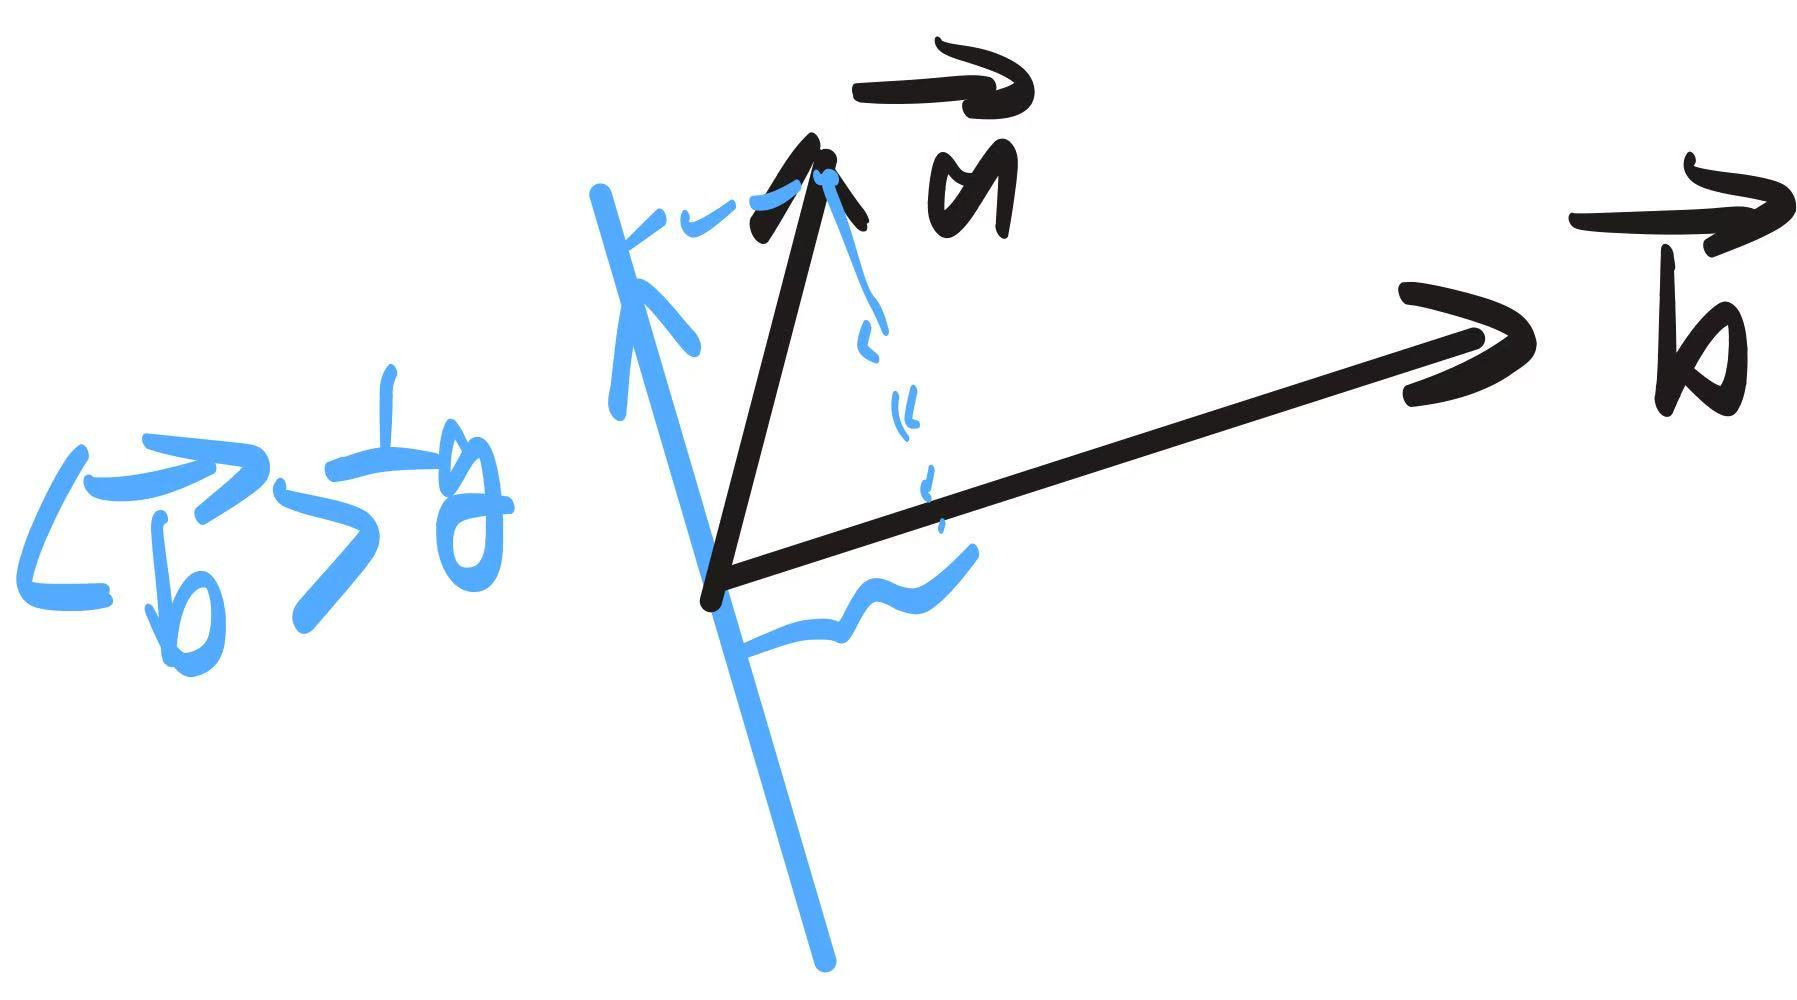
\includegraphics[height=2cm]{chapters/08/O-p}
          \begin{flalign*}
              \text{pr}_{\overrightarrow{b}}:\, V                               & \to \left\langle\overrightarrow{b}\right\rangle                                                                                                                               & \\
              \overrightarrow{a}                                                & \mapsto\frac{\left\langle\overrightarrow{a},\overrightarrow{b}\right\rangle_g}{\left|\overrightarrow{b}\right|_g}\frac{\overrightarrow{b}}{\left|\overrightarrow{b}\right|_g} & \\
              \text{pr}_{\left\langle\overrightarrow{b}\right\rangle^\perp}:\,V & \to\left\langle\overrightarrow{b}\right\rangle^{\perp_g}\text{ (orthogonal complement)}                                                                                       & \\
              \overrightarrow{a}                                                & \mapsto\overrightarrow{a}-\text{pr}_{\overrightarrow{b}}\overrightarrow{a}                                                                                                    &
          \end{flalign*}
          \emph{$V=\left\langle\overrightarrow{b}\right\rangle\oplus \left\langle\overrightarrow{b}\right\rangle^{\perp_g}$}
    \item Volume of a ``$k$-dimensional'' parallelepiped 平行多面体 is defined inductively.\\
          The set $P_{v_1,\dots,v_k}=\left\{\sum_{i=1}^k t_i v_i\mid 0\leq t_1,\dots,t_k\leq 1\right\}$ is called the parallelepiped spanned by $\left(v_1,\dots,v_k\right)$ in $V$.
          \begin{itemize}
              \item $k=1,\,\text{Vol}_g\left(P_v\right)=|v|_g$
              \item $k=2,\,\text{Vol}_g\left(P_{v_1,v_2}\right)\triangleq \text{Vol}_g\left(P_{v_1}\right)\left|\text{pr}_{\left\langle v_1\right\rangle^{\perp_g}}v_2\right|_g$
          \end{itemize}
          \begin{flalign*}
              \text{Vol}_g\left(P_{v_1,v_2}\right)^2 & =\left|v_1\right|_g^2\left(\left|v_2\right|_g^2-\left(\frac{\left\langle v_1,v_2\right\rangle_g}{\left|v_1\right|_g}\right)^2\right) & \\
                                                     & =\left|v_1\right|_g^2\left|v_2\right|_g^2-\left\langle v_1,v_2\right\rangle_g^2                                                      & \\
                                                     & =  \det\begin{pmatrix}
                                                                  \left\langle v_1,v_1\right\rangle_g & \left\langle v_1,v_2\right\rangle_g \\
                                                                  \left\langle v_2,v_1\right\rangle_g & \left\langle v_2,v_2\right\rangle_g
                                                              \end{pmatrix}                                                         &
          \end{flalign*}
          \emph{$v_2=\text{pr}_{v_1}v_2+\text{pr}_{v_1^{\perp_g}}v_2$\\$\left|v_2\right|_g^2=\left|\text{pr}_{v_1}v_2\right|_g^2+\left|\text{pr}_{v_1^{\perp_g}}v_2\right|_g^2$}
\end{enumerate}

\begin{theorem}
    $\text{Vol}_g\left(P_{v_1,\dots,v_k}\right)=\sqrt{\det\left(\left\langle v_i,v_j\right\rangle_g\right)}$
\end{theorem}

\subsubsection{Orientation 定向}

\begin{definition}[Equivalence Relation]
    A subset $S\subseteq X\times X=\left\{(x,y)\mid x\in X,y\in X\right\}$ is called a binary relation on $X$. A binary relation $S$ on $X$ is called an \allbold{equivalence relation 等价关系} on $X$ if
    \begin{enumerate}
        \item Symmetry: $(x,y)\in S\Rightarrow (y,x)\in S$
        \item Transitivity: $(x,y)\in S,\,(y,z)\in S\Rightarrow (x,z)\in S$
        \item Reflexivity: $(x,x)\in S,\,\forall x\in X$
    \end{enumerate}
    It is usually denoted by ``$\sim_S$'' or ``$\sim$''.
\end{definition}

\begin{definition}[Equivalence Class]
    Let ``$\sim$'' be an equivalence relation on $X$. Then for any $x\in X$, the set $\left\{y\in X\mid y\sim x\right\}\subseteq X$ is called an equivalence class, denoted by $[x]_\sim$. Any $y\in[x]_\sim$ is called a representative of $[x]_\sim$. $X/_\sim\triangleq \left\{[x]_\sim\mid x\in X\right\}$ is called the quotient set of $X$ under the relation ``$\sim$''.
\end{definition}

\begin{example}
    \begin{enumerate}
        \item $\left\{(x,y)\in\mathbb{R}^2\mid x>y \right\}$ (``$>$'') is a binary relation on $\mathbb{R}$, but not an equivalence relation.
        \item $S=\Delta x=\left\{(x,x)\mid x\in X\right\}$ (``$=$'') is an equivalence relation.
        \item (Congruence) Fix $n\in\mathbb{N}$
              $$\left\{(x,y)\in\mathbb{Z}\times\mathbb{Z}\mid n\mid(x-y)\right\}$$
              This equivalence relation is called ``$\bmod n$ congruence'' ($\equiv\,\bmod n$).

              $\mathbb{Z}/_{\equiv n}\left(\triangleq\mathbb{Z}_n\right)=\left\{[0]_{\equiv n},\dots,[n-1]_{\equiv n}\right\}$\\
              \allbold{$\mathbb{Z}_2=\left\{[0]_{\equiv 2},[1]_{\equiv 2}\right\}$}

              $[k]_{\equiv n}=\left\{l\in\mathbb{Z}\mid n\mid(l-k)\right\}=\left\{k+mn\mid m\in\mathbb{Z}\right\}$ is called the ``$\bmod n$ congruence class of $k$''.
    \end{enumerate}
\end{example}

\hrule

\begin{example}
    \begin{enumerate}
        \item $X=\left\{\text{triangle on }\mathbb{R}^2\right\}\ \cong\ \simeq $
              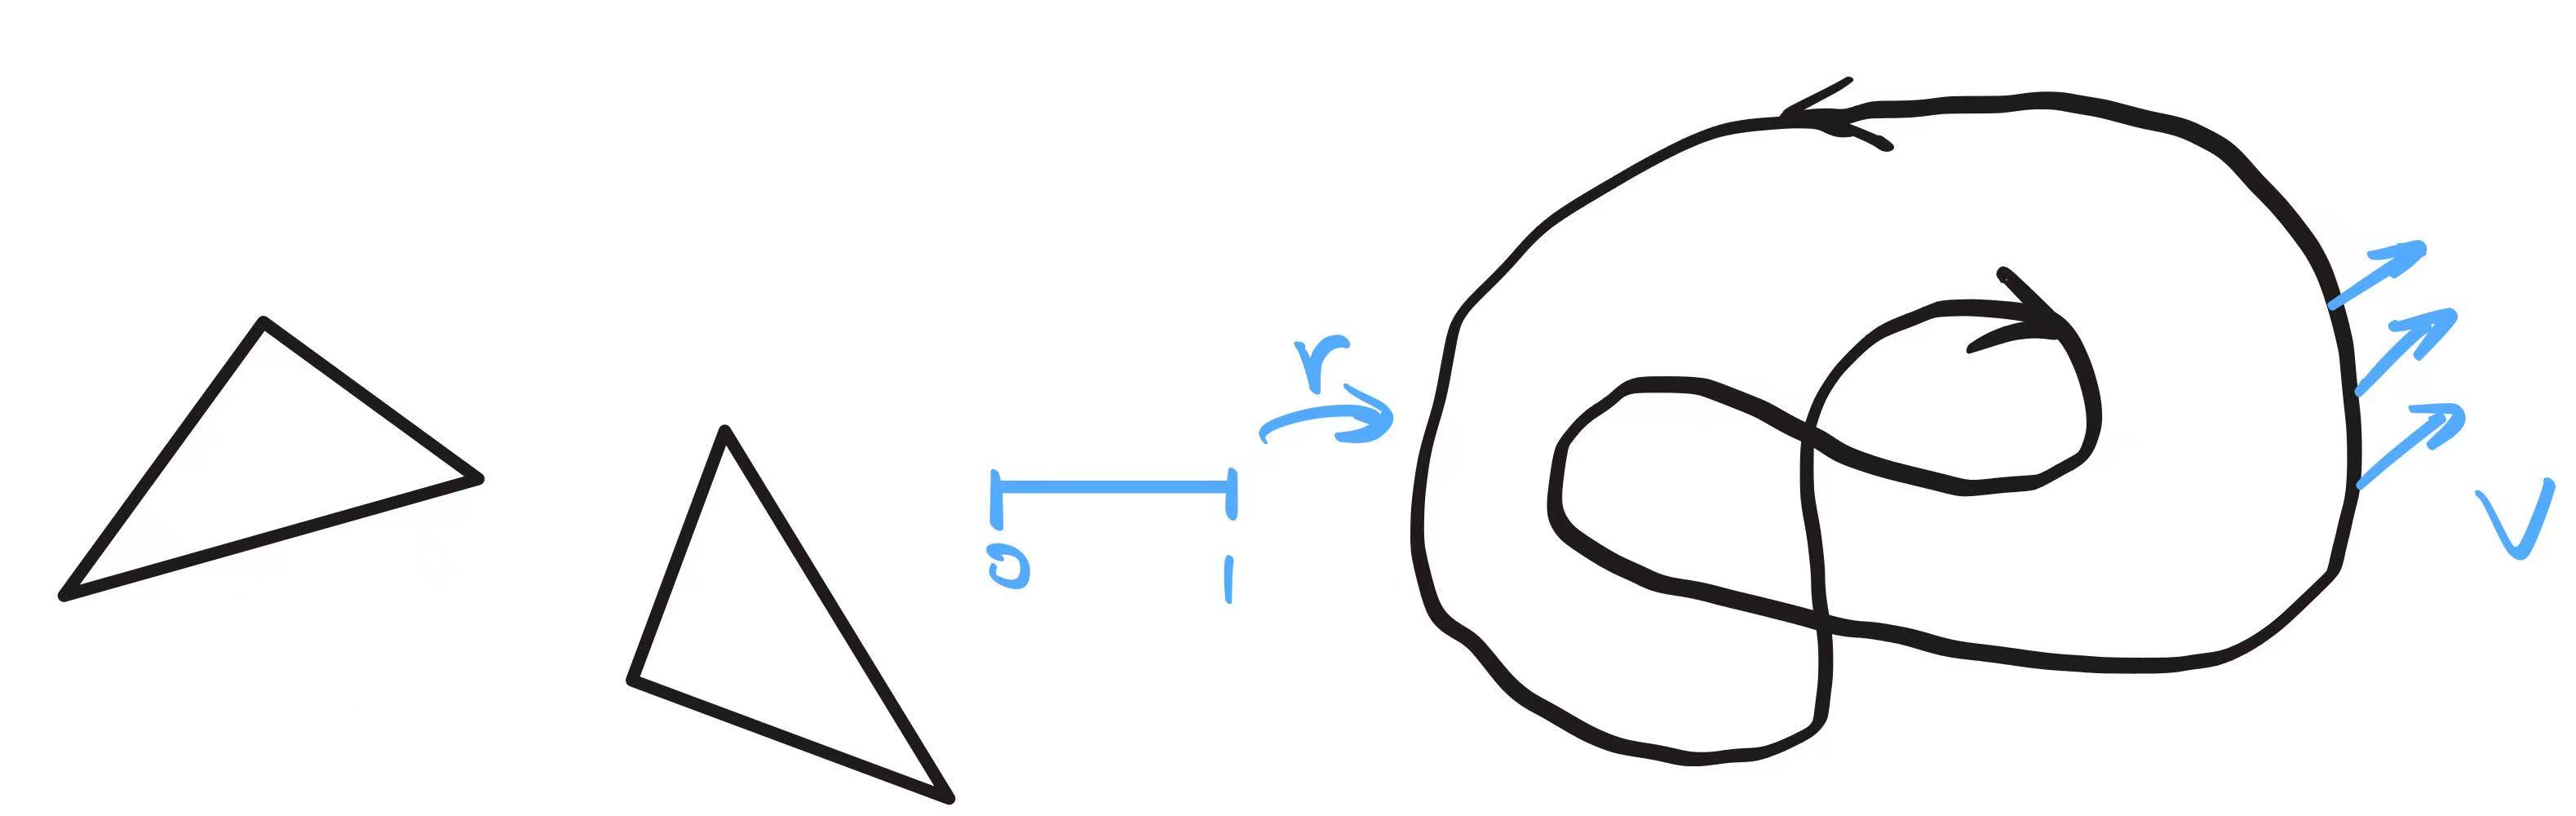
\includegraphics[height=2cm]{chapters/08/sim}
        \item Similarity of matrices: $A\sim B\iff A=PBP^{-1}$ for some $P\in\text{GL}(n,\mathbb{R})$.
              $$M_{n\times n}(\mathbb{R})/_\sim=\left\{\text{Jordan canonical form}\right\}$$
    \end{enumerate}
\end{example}

\begin{definition}[Orientation \emph{定向}, Oriented Vector Space \emph{定向线性空间}]
    Let $\mathcal{B}_V=\left\{\text{ordered bases of }V\right\}$ where $V$ is a real vector space. Define
    $$\left(v_1',\dots,v_n'\right)=\left(v_1,\dots,v_n\right)P$$
    for some $P\in\text{GL}(n,\mathbb{R}),\,\det P>0$ iff $\left(v_1',\dots,v_n'\right)\sim\left(v_1,\dots,v_n\right)$.

    This is an equivalence relation, and $\mathcal{B}_V/_\sim=\left\{o_1,o_2\right\}$. An element of $\mathcal{B}_V/_\sim$ is called an \emph{orientation} on $V$. Any vector space, together with a choice of orientation, is called an \emph{oriented vector space}.
\end{definition}

\subsubsection{$\mathbb{R}^n$: Euclidean Space}
Equipped with the standard inner product
$$\langle x,y\rangle=\sum_{i=1}^n x_iy_i$$
where $x=\left(x_1,\dots,x_n\right)^+,y=\left(y_1,\dots,y_n\right)^+\in\mathbb{R}^n$.

Under this inner product, $\left(e_1,\dots,e_n\right)$, where $e_i=(0,\dots,0,\overset{i}{1},0,\dots,0)$, is called the \emph{standard} orthonormal basis.

\begin{remark}
    $n=2$, $\left(e_1,e_2\right)$ is usually denoted by $i,j$;

    $n=3$, $\left(e_1,e_2,e_3\right)$ is denoted by $i,j,k$
\end{remark}

\begin{definition}[Cross Product in $\mathbb{R}^3$]
    Let $x,y\in\mathbb{R}^3$. Define ``$\times$'' by
    \begin{align*}
        x\times y & =
        \begin{vmatrix}
            i   & j   & k   \\
            x_1 & x_2 & x_3 \\
            y_1 & y_2 & y_3
        \end{vmatrix}=
        \begin{vmatrix}
            x_2 & x_3 \\
            y_2 & y_3
        \end{vmatrix}i-
        \begin{vmatrix}
            x_1 & x_3 \\
            y_1 & y_3
        \end{vmatrix}j+
        \begin{vmatrix}
            x_1 & x_2 \\
            y_1 & y_2
        \end{vmatrix}k                                                  \\
                  & =(x_2y_3-x_3y_2)i+(x_3y_1-x_1y_3)j+(x_1y_2-x_2y_1)k
    \end{align*}
    This is called the cross product of $x$ and $y$.
\end{definition}

\begin{proposition}
    \begin{enumerate}
        \item $x\times y=-(y\times x)$ \emph{($x\times y=0\iff\{x,y\}$ are linearly dependent)} (anti-symmetry)
        \item $(\lambda x+\mu y)\times z=\lambda x\times z+\mu y\times z$ (Bilinear)
        \item $\langle x\times y,x\rangle=0$, $\langle x\times y,y\rangle=0$; $(x,y,x\times y)$ determines the same orientation as $(i,j,k)$
        \item $|x\times y|=\text{Area}\left(P_{x,y}\right)$
    \end{enumerate}
\end{proposition}

\begin{pf}
    \begin{enumerate}[start=3]
        \item \begin{align*}
                  (x,y,x\times y) & =(i,j,k)\begin{pmatrix}
                                                x_1 & y_1 & \begin{vmatrix}
                                      x_2 & y_2 \\
                                      x_3 & y_3
                                  \end{vmatrix} \\
                                                x_2 & y_2 & \begin{vmatrix}
                                      x_3 & y_3 \\
                                      x_1 & y_1
                                  \end{vmatrix} \\
                                                x_3 & y_3 & \begin{vmatrix}
                                      x_1 & y_1 \\
                                      x_2 & y_2
                                  \end{vmatrix}
                                            \end{pmatrix} \\
                                  & =|x\times y|^2
              \end{align*}
              $\implies$ if $\{x,y\}$ are linearly independent, $(x,y,x\times y)$ has the same orientation as $(i,j,k)$.
              \begin{remark}
                  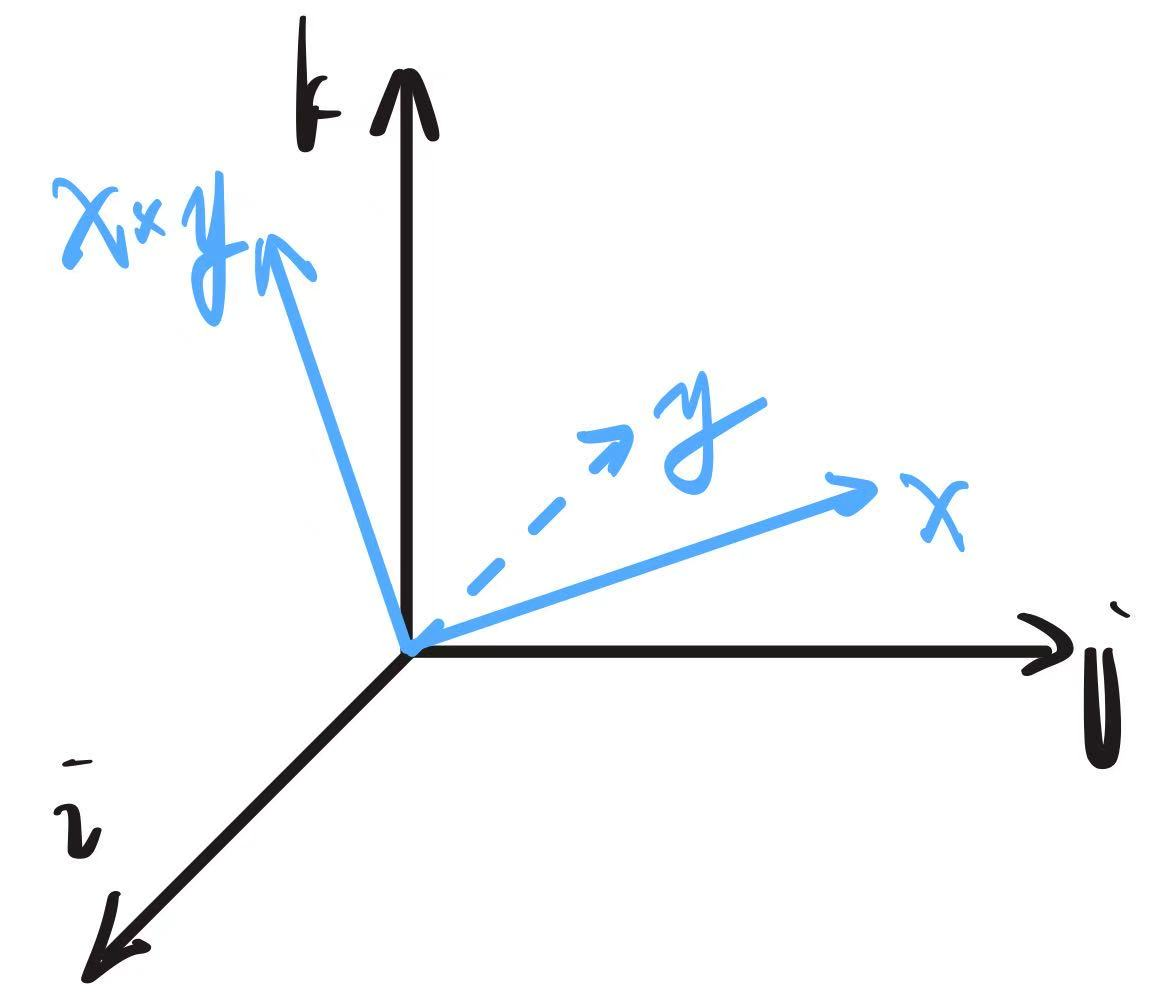
\includegraphics[height=2cm]{chapters/08/xprop3pf}
                  \begin{itemize}
                      \item The orientation denoted by $(i,j,k)$ is called right-hand orientation;
                      \item The orientation denoted by $(i,j,-k)$ is called left-hand orientation;
                      \item The ordered basis with the Right-Hand orientation is called a Right-Hand system.
                  \end{itemize}
              \end{remark}
        \item \begin{align*}
                  |x\times y|^2                     & =\left(x_2y_3-x_3y_2\right)^2+\left(x_3y_1-x_1y_3\right)^2+\left(x_1y_2-x_2y_1\right)^2           \\
                  \text{Area}\left(P_{x,y}\right)^2 & =\det\begin{pmatrix}
                                                               \langle x,x\rangle & \langle x,y\rangle \\
                                                               \langle y,x\rangle & \langle y,y\rangle
                                                           \end{pmatrix}                                                      \\
                                                    & =\left(x_1^2+x_2^2+x_3^2\right)\left(y_1^2+y_2^2+y_3^2\right)-\left(x_1y_1+x_2y_2+x_3y_3\right)^2
              \end{align*}
              \begin{theorem}
                  \allbold{In $\mathbb{R}^3$, the cross product is uniquely determined by the four properties.}

                  \raisebox{-0.5\height}{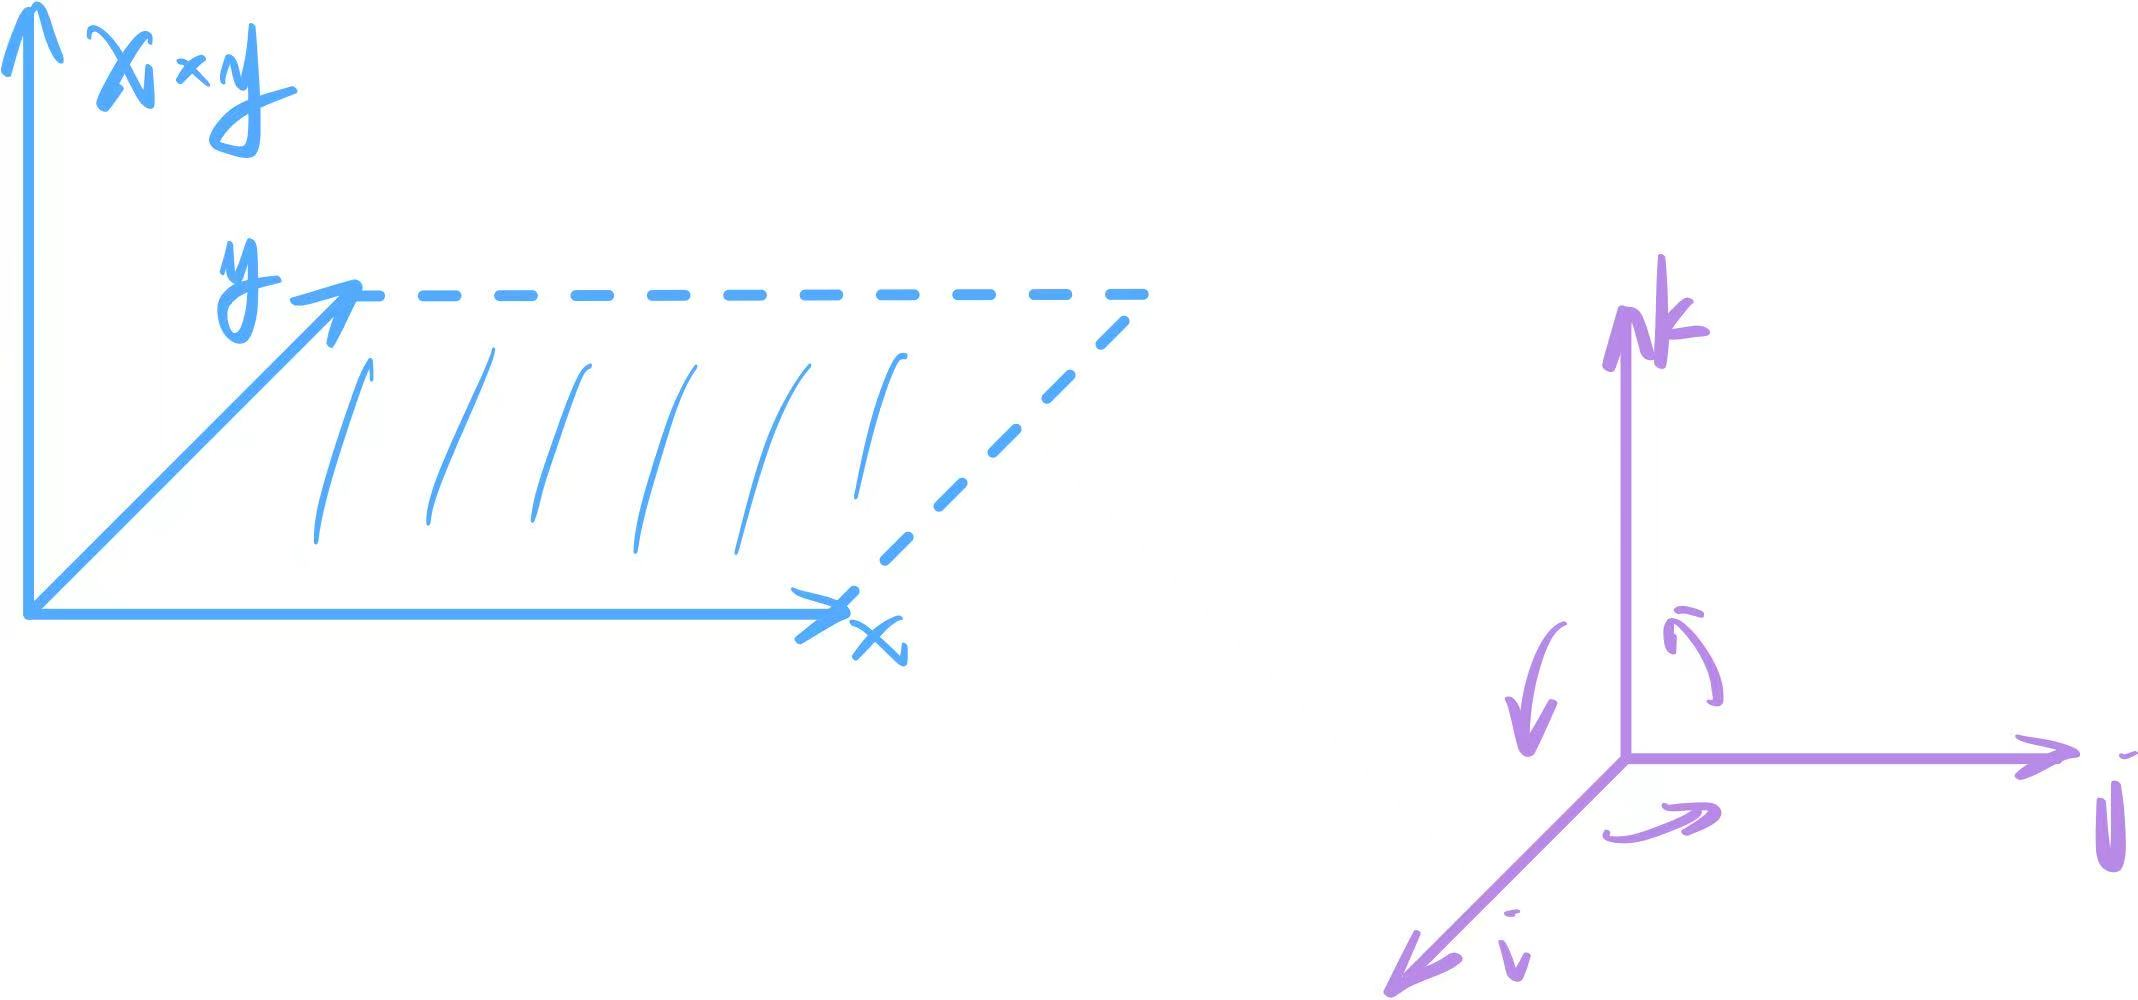
\includegraphics[height=2cm]{chapters/08/xprop4pf}}$\begin{cases}
                          i\times j=k \\
                          j\times k=i \\
                          k\times i=j
                      \end{cases}\implies x\times y=\cdots$
              \end{theorem}
    \end{enumerate}
\end{pf}

\begin{definition}[Mixed Product on $\mathbb{R}^3$ 混合积]
    Let $a,b,c\in\mathbb{R}^3$.

    $$\langle a,b\times c\rangle=\langle b,c\times a\rangle=\langle c,a\times b\rangle=\begin{vmatrix}
            a_1 & a_2 & a_3 \\
            b_1 & b_2 & b_3 \\
            c_1 & c_2 & c_3
        \end{vmatrix}$$
    \raisebox{-0.5\height}{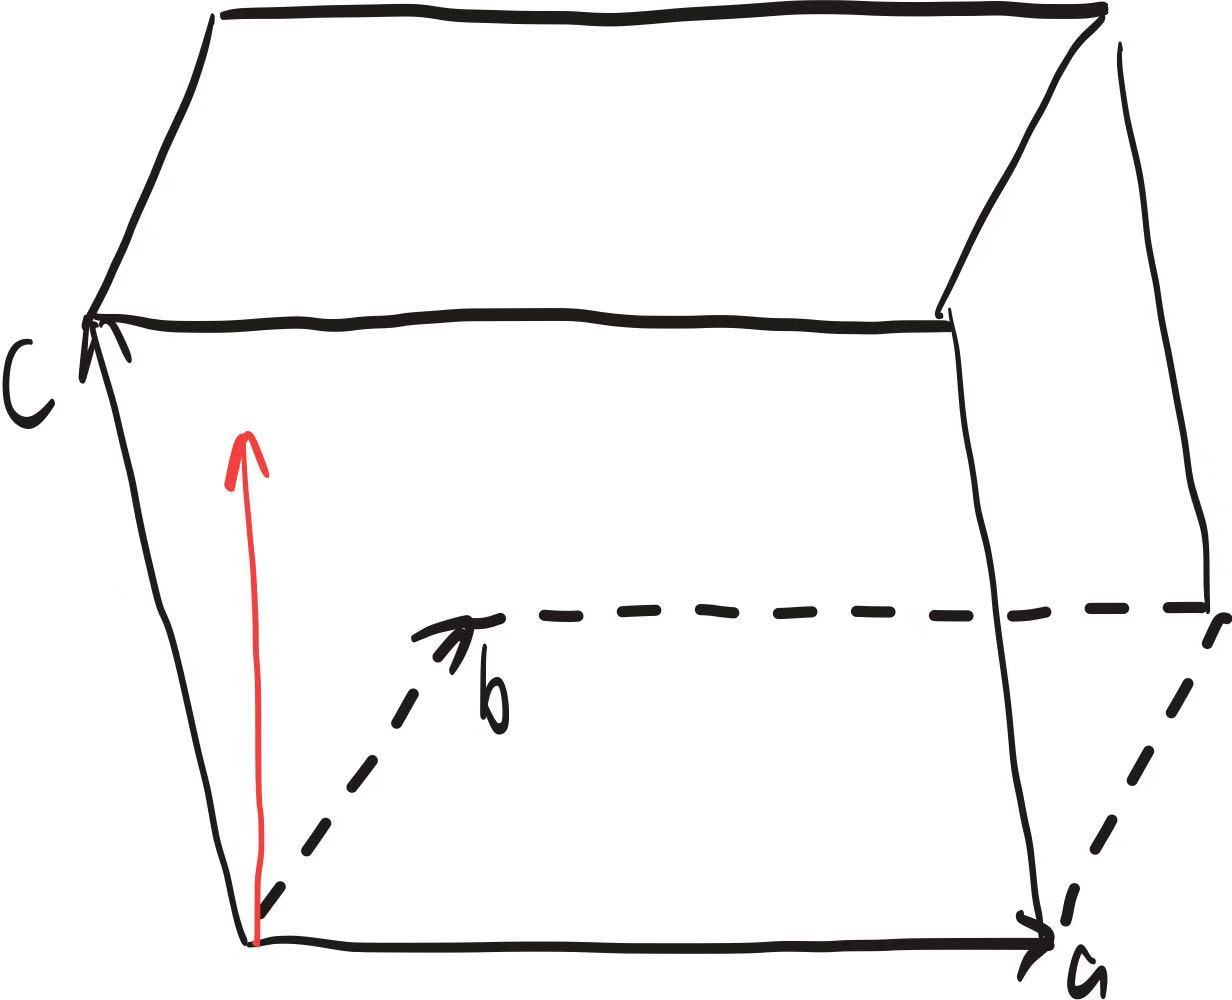
\includegraphics[height=2cm]{chapters/08/mixproduct}}

    is called the mixed product of $a,b,c$.
    \begin{itemize}
        \item $\langle c,a\times b\rangle$ measures the ``\allbold{signed volume}'' of $P_{a,b,c}$;
        \item This equation also gives the formula for the volume of a parallelepiped in $\mathbb{R}^3$;
        \item \allbold{$\left\langle c,a\times b\right\rangle\begin{cases}
                          >0 & (a,b,c)\text{ is a Right-Hand system} \\
                          =0 & \{a,b,c\}\text{ linearly dependent}   \\
                          <0 & (a,b,c)\text{ is a Left-Hand system}
                      \end{cases}$}
    \end{itemize}
\end{definition}

\allbold{Recall:}

$\text{Vol}\left(P_{v_1,\dots,v_k}\right)=\sqrt{\det\left(\left\langle v_i,v_j\right\rangle\right)},\,v_1,\dots,v_k\in\mathbb{R}^n$

If
$$v_i=\sum_{s=1}^n e_s\underset{\substack{\downarrow\\\emph{Coordinate vector for $v_i$}}}{P_{s_i}}\quad\left(\iff\left(v_1,\dots,v_k\right)=\left(e_1,\dots,e_n\right)P\right),$$
then
\begin{align*}
    \left\langle v_i,v_j\right\rangle & =\left\langle\sum_{s=1}^n e_s P_{s_i}, \sum_{t=1}^n e_t P_{t_j}\right\rangle
    =\sum_{s,t=1}^n P_{s_i}P_{t_j}\delta_{st}
    =\sum_{s=1}^n P_{s_i}P_{s_j}                                                                                     \\
                                      & =\left(P^TP\right)_{ij}
\end{align*}

\emph{$\implies\text{Vol}\left(P_{v_1,\dots,v_k}\right)=\sqrt{\det\left(P^TP\right)}$}

\allbold{($\implies$ In $\mathbb{R}^3$, $\text{Vol}\left(P_{a,b,c}\right)=\sqrt{\det\left(P^TP\right)}=\sqrt{\left(\det P\right)^2}=\left|\det P\right|$)}

\begin{theorem}[Cauchy-Binet]
    $$\det\left(U^TU\right)=\sum_{\underset{\begin{pmatrix}n\\k\end{pmatrix}}{1\leq i_1<\dots<i_k\leq n}}U\begin{pmatrix}
            i_1 & \dots & i_k \\
            1   & \dots & k
        \end{pmatrix}^2$$
    \emph{$$U^TU=\begin{pmatrix}
                U_{11} & \cdots                       & U_{n1} \\
                \vdots &                              & \vdots \\
                U_{1k} & \underset{\substack{\uparrow          \\i_1\,i_k}}{\cdots}&U_{nk}
            \end{pmatrix}\begin{pmatrix}
                U_{11} & \cdots & U_{1k} &                     \\
                \vdots &        & \vdots & \leftarrow i_1\,i_k \\
                U_{n1} & \cdots & U_{nk} &
            \end{pmatrix}$$}
\end{theorem}

\begin{corollary}[Generalized Pythagorean Theorem]
    $$\text{Vol}\left(P_{v_1,\dots,v_k}\right)^2=\sum_{1\leq i_1<\dots<i_k\leq n}U\begin{pmatrix}
            i_1 & \dots & i_k \\
            1   & \dots & k
        \end{pmatrix}^2\,(k=1,\,|V|^2=\left\langle V,e_1\right\rangle^2+\dots+\left\langle V,e_n\right\rangle^2)$$
\end{corollary}